\documentclass[a4paper,14pt]{article}

%%% Работа с русским языком
\usepackage{cmap}					% поиск в PDF
\usepackage{mathtext} 				% русские буквы в формулах
\usepackage[T2A]{fontenc}			% кодировка
\usepackage[utf8]{inputenc}			% кодировка исходного текста
\usepackage[english,russian]{babel}	% локализация и переносы
\usepackage{indentfirst}
\usepackage{caption}
\frenchspacing

\renewcommand{\epsilon}{\ensuremath{\varepsilon}}
\renewcommand{\phi}{\ensuremath{\varphi}}
\renewcommand{\kappa}{\ensuremath{\varkappa}}
\renewcommand{\le}{\ensuremath{\leqslant}}
\renewcommand{\leq}{\ensuremath{\leqslant}}
\renewcommand{\ge}{\ensuremath{\geqslant}}
\renewcommand{\geq}{\ensuremath{\geqslant}}
\renewcommand{\emptyset}{\varnothing}

\newcommand{\T}{^{\mathsf{T}}}
\newcommand{\uX}{\ensuremath{\underline{X}}}
\newcommand{\bx}{\mathbf{x}}
\newcommand{\by}{\mathbf{y}}
\newcommand{\bX}{\mathbf{X}}
\newcommand{\bY}{\mathbf{Y}}
\newcommand{\bH}{\mathbf{H}}
\newcommand{\dH}{\mathbb{H}}

%%% Дополнительная работа с математикой
\usepackage{amsmath,amsfonts,amssymb,amsthm,mathtools,dsfont} % AMS
\usepackage{icomma} % "Умная" запятая: $0,2$ --- число, $0, 2$ --- перечисление

%% Номера формул
%\mathtoolsset{showonlyrefs=true} % Показывать номера только у тех формул, на которые есть \eqref{} в тексте.
%\usepackage{leqno} % Нумереация формул слева

%% Свои команды
\DeclareMathOperator{\sgn}{\mathop{sgn}}

%% Перенос знаков в формулах (по Львовскому)
\newcommand*{\hm}[1]{#1\nobreak\discretionary{}
	{\hbox{$\mathsurround=0pt #1$}}{}}

%%% Работа с картинками
\usepackage{graphicx}  % Для вставки рисунков
\setlength\fboxsep{3pt} % Отступ рамки \fbox{} от рисунка
\setlength\fboxrule{1pt} % Толщина линий рамки \fbox{}
\usepackage{wrapfig} % Обтекание рисунков текстом
\usepackage{subfigure}

%%% Работа с таблицами
\usepackage{array,tabularx,tabulary,booktabs} % Дополнительная работа с таблицами
\usepackage{longtable}  % Длинные таблицы
\usepackage{multirow} % Слияние строк в таблице

%%% Теоремы
\theoremstyle{plain} % Это стиль по умолчанию, его можно не переопределять.
\newtheorem{theorem}{Теорема}[section]
\newtheorem{proposition}[theorem]{Утверждение}
\newtheorem{definition}{Определение}

\theoremstyle{definition} % "Определение"
\newtheorem{corollary}{Следствие}[theorem]
\newtheorem{problem}{Задача}[section]

\theoremstyle{remark} % "Примечание"
\newtheorem*{nonum}{Решение}

%%% Программирование
\usepackage{etoolbox} % логические операторы

%%% Страница
\usepackage{extsizes} % Возможность сделать 14-й шрифт
\usepackage{geometry} % Простой способ задавать поля
\geometry{top=25mm}
\geometry{bottom=35mm}
\geometry{left=35mm}
\geometry{right=20mm}
%
%\usepackage{fancyhdr} % Колонтитулы
% 	\pagestyle{fancy}
%\renewcommand{\headrulewidth}{0pt}  % Толщина линейки, отчеркивающей верхний колонтитул
% 	\lfoot{Нижний левый}
% 	\rfoot{Нижний правый}
% 	\rhead{Верхний правый}
% 	\chead{Верхний в центре}
% 	\lhead{Верхний левый}
%	\cfoot{Нижний в центре} % По умолчанию здесь номер страницы

\usepackage{setspace} % Интерлиньяж
%\onehalfspacing % Интерлиньяж 1.5
%\doublespacing % Интерлиньяж 2
%\singlespacing % Интерлиньяж 1

\usepackage{lastpage} % Узнать, сколько всего страниц в документе.

\usepackage{soul} % Модификаторы начертания

\usepackage{hyperref}
\usepackage[usenames,dvipsnames,svgnames,table,rgb]{xcolor}
\hypersetup{				% Гиперссылки
	unicode=true,           % русские буквы в раздела PDF
	pdftitle={Заголовок},   % Заголовок
	pdfauthor={Автор},      % Автор
	pdfsubject={Тема},      % Тема
	pdfcreator={Создатель}, % Создатель
	pdfproducer={Производитель}, % Производитель
	pdfkeywords={keyword1} {key2} {key3}, % Ключевые слова
	colorlinks=true,       	% false: ссылки в рамках; true: цветные ссылки
	linkcolor=red,          % внутренние ссылки
	citecolor=black,        % на библиографию
	filecolor=magenta,      % на файлы
	urlcolor=cyan           % на URL
}

\usepackage{csquotes} % Еще инструменты для ссылок

%\usepackage[style=authoryear,maxcitenames=2,backend=biber,sorting=nty]{biblatex}

\usepackage{multicol} % Несколько колонок

\usepackage{tikz} % Работа с графикой
\usepackage{pgfplots}
\usepackage{pgfplotstable}


\author{Владимиров Эдуард, группа Б05-928}
\title{\textbf{Отчёт о лабораторной работе №2}}
\date{\today}

\begin{document}
	\maketitle

	\section{Введение}
	Цель лабораторной работы заключается в применении метода HOSVD для снижения размерности кадров gif-изображения и использовании метода CCM для обнаружения связи между картинками и звуком.  
	Эксперимент проводится на 15-кадровом черно-белом мультфильме с идущей уткой и сгенерированным звуковым рядом.
	
	Ссылка на код: \href{https://github.com/intsystems/MathematicalForecastingMethods/blob/main/lab2/vladimirov/lab2.ipynb}{тык}
	
	\section{Постановка задачи}
	Введём обозначения:  
	
	$\uX \in \mathds{R}^{N \times I \times J}$ - временной ряд кадров: число кадров $\cdot$ размеры изображения
	
	$Y \in \mathds{R}^N$ - временной ряд звуков
	
	Наша цель заключается в определении наличия связи $\uX \rightarrow Y$. Строгое математическое правило для этого будет предъявлено ниже.
	
	\subsection{HOSVD}
	Мы можем расписать $\uX$ как: 
	\begin{gather*}
		\uX \cong \sum_{t=1}^{N} \sum_{i=1}^{R_i} \sum_{j=1}^{R_j} \sigma_{t i j} (u^{(1)}_t \circ u^{(2)}_i \circ u^{(3)}_j),
	\end{gather*}
	где $\circ$ ~--- это внешнее произведение и 
	\begin{gather*}
		U^{(1)} = \left[ u^{(1)}_{1}, \dots , u^{(1)}_{N} \right],
		U^{(2)} = \left[ u^{(2)}_{1}, \dots , u^{(2)}_{R_i} \right], 
		U^{(3)} = \left[ u^{(3)}_{1}, \dots , u^{(3)}_{R_j} \right].
	\end{gather*}
	
	\begin{figure}[bhtp]
		\centering
		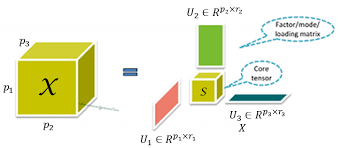
\includegraphics[width=\linewidth]{hosvd-2.png}
		\caption{Иллюстрация метода HOPLS}
	\end{figure}
	
	Или в обозначениях Такера:
	\begin{gather*}
		\underline{X} \cong \underline{G} \times_{1} U^{(1)} \times_{2} U^{(2)} \times_{3} U^{(3)}, \\
		[G]_{t i j} = \sigma_{t i j} \text{~--- core-тензор,} \\
		\underline{G} \in \mathds{R}^{N \times R_i \times R_j},
	\end{gather*}
	где $\times_{i}$ ~--- операция матрично-тензорного умножения.

	\begin{figure}[bhtp]
		\centering
		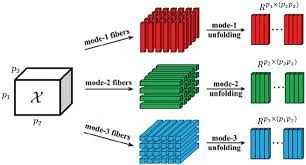
\includegraphics[width=\linewidth]{hosvd-1.jpeg}
		\caption{Матризация тензора $\uX$, использующая в операция матрично-тензорного умножения $\times_l$}
	\end{figure}

	\subsection{CCM}
	Из апроксимированного тензора $\underline{X}$ и $Y$ составим их многомерные траекторные матрицы, считая период движения равным $T$:
	\begin{gather*}
		\bH_X \in \mathbb{R}^{(N-T+1) \times T \times I \times J}, \\
		\bH_Y \in \mathbb{R}^{(N-T+1) \times T},
	\end{gather*}

	Определим отображение из траекторного пр-ва звукового сигнала $\dH_Y \in \mathds{R}^{T}$ в траекторное пространство кадров $\dH_X \in \mathds{R}^{T \times I \times J}$ следующим образом:
	
	$$ \varphi: \by_0 \mapsto \widehat{\bx_0} = \sum\limits_{i=1}^K w_i \bx_i, \qquad 
	w_i = \dfrac{u_i}{\sum\limits_{j=1}^K u_j}, \qquad
	u_i = \exp \bigl( - \| \by_0 - \by_i \| \bigr).$$
	
	В работе будет рассмотрено два определения наличия связи между временными рядами:
	\begin{enumerate}
		\item Липшицевость отображения $\varphi$:
		$$\rho_{\dH_X}(\varphi(\by_i), \varphi(\by_j)) \leq C \rho_{\dH_Y}(\by_i, \by_j) \qquad \by_i, \by_j \in \dH_Y. $$
		$$ \dfrac{\rho_{\dH_Y}(\mathbf{y}_i, \mathbf{y}_j)}{\rho_{\dH_X}(\varphi(\mathbf{y}_i),  \varphi(\mathbf{y}_j))} \geqslant C^{-1}$$
		\item Высокая корреляция между $\widehat{\bx_0}$ и $\bx_0$
	\end{enumerate} 
	
	\section{Вычислительный эксперимент}
	\begin{figure}
		\centering
		\subfigure[]{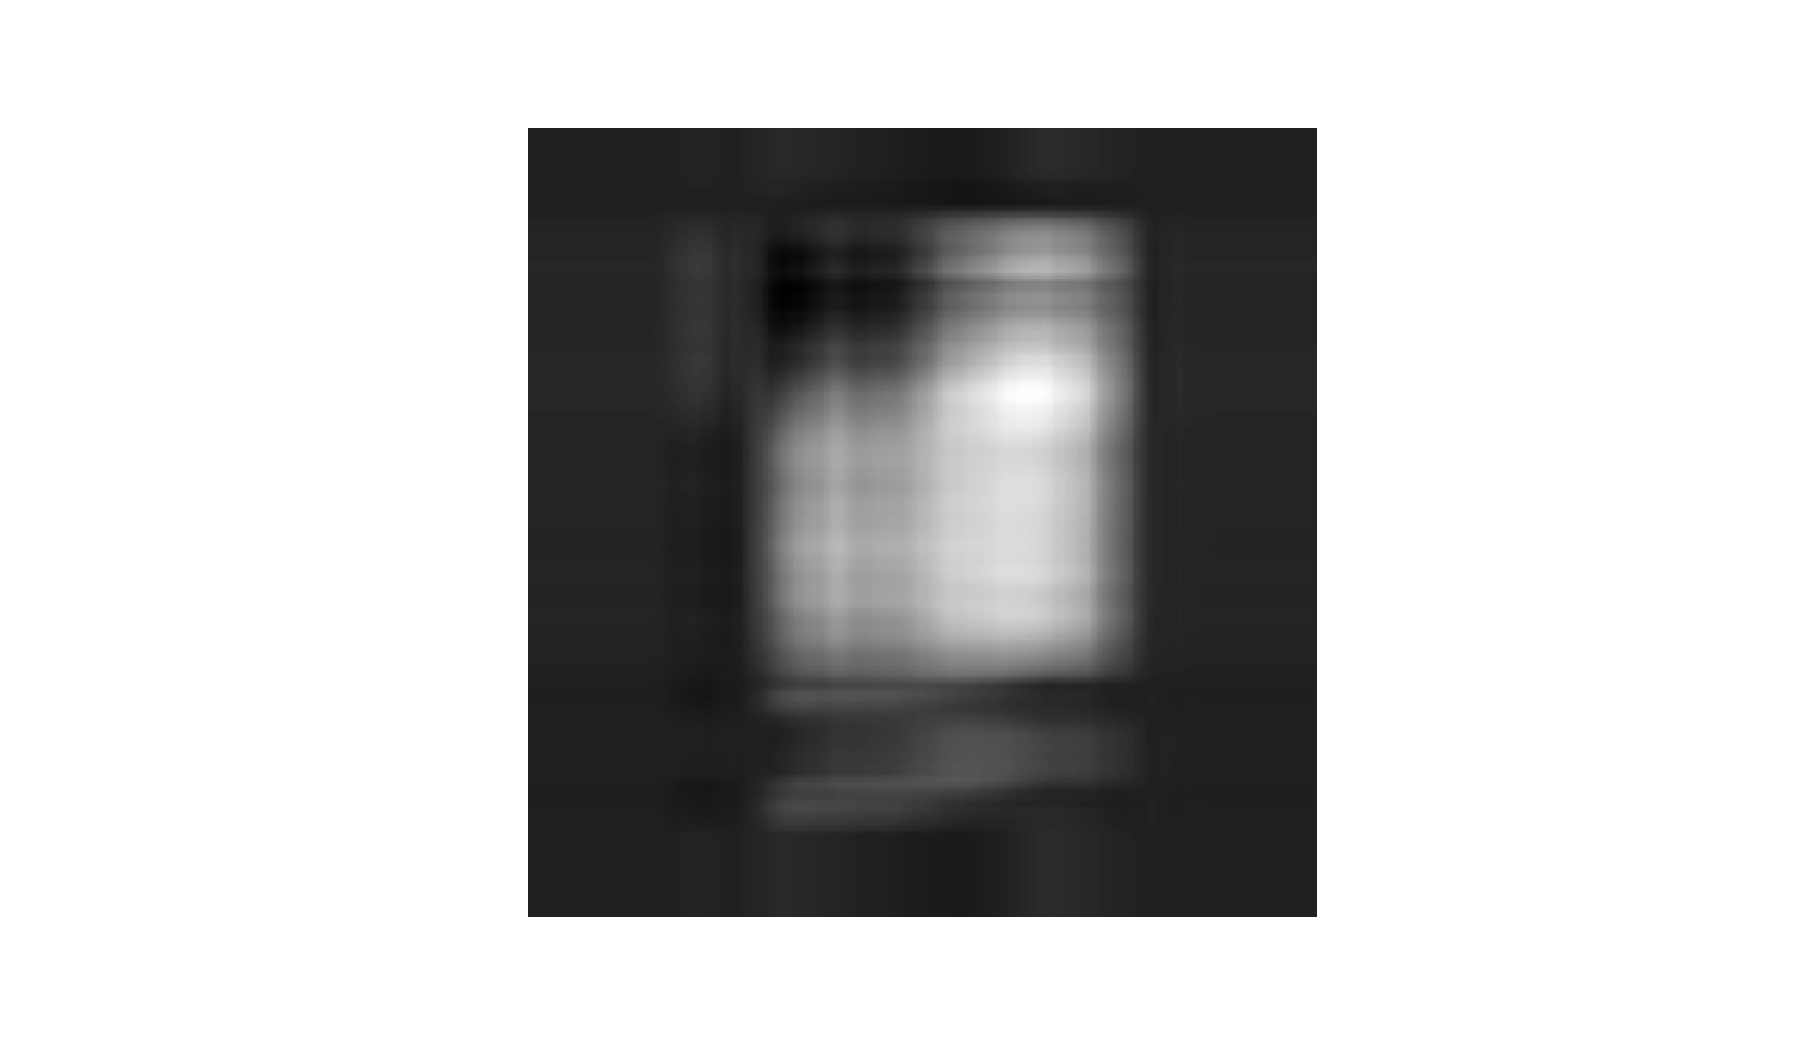
\includegraphics[width=0.32\textwidth]{../approx_4.pdf}} 
		\subfigure[]{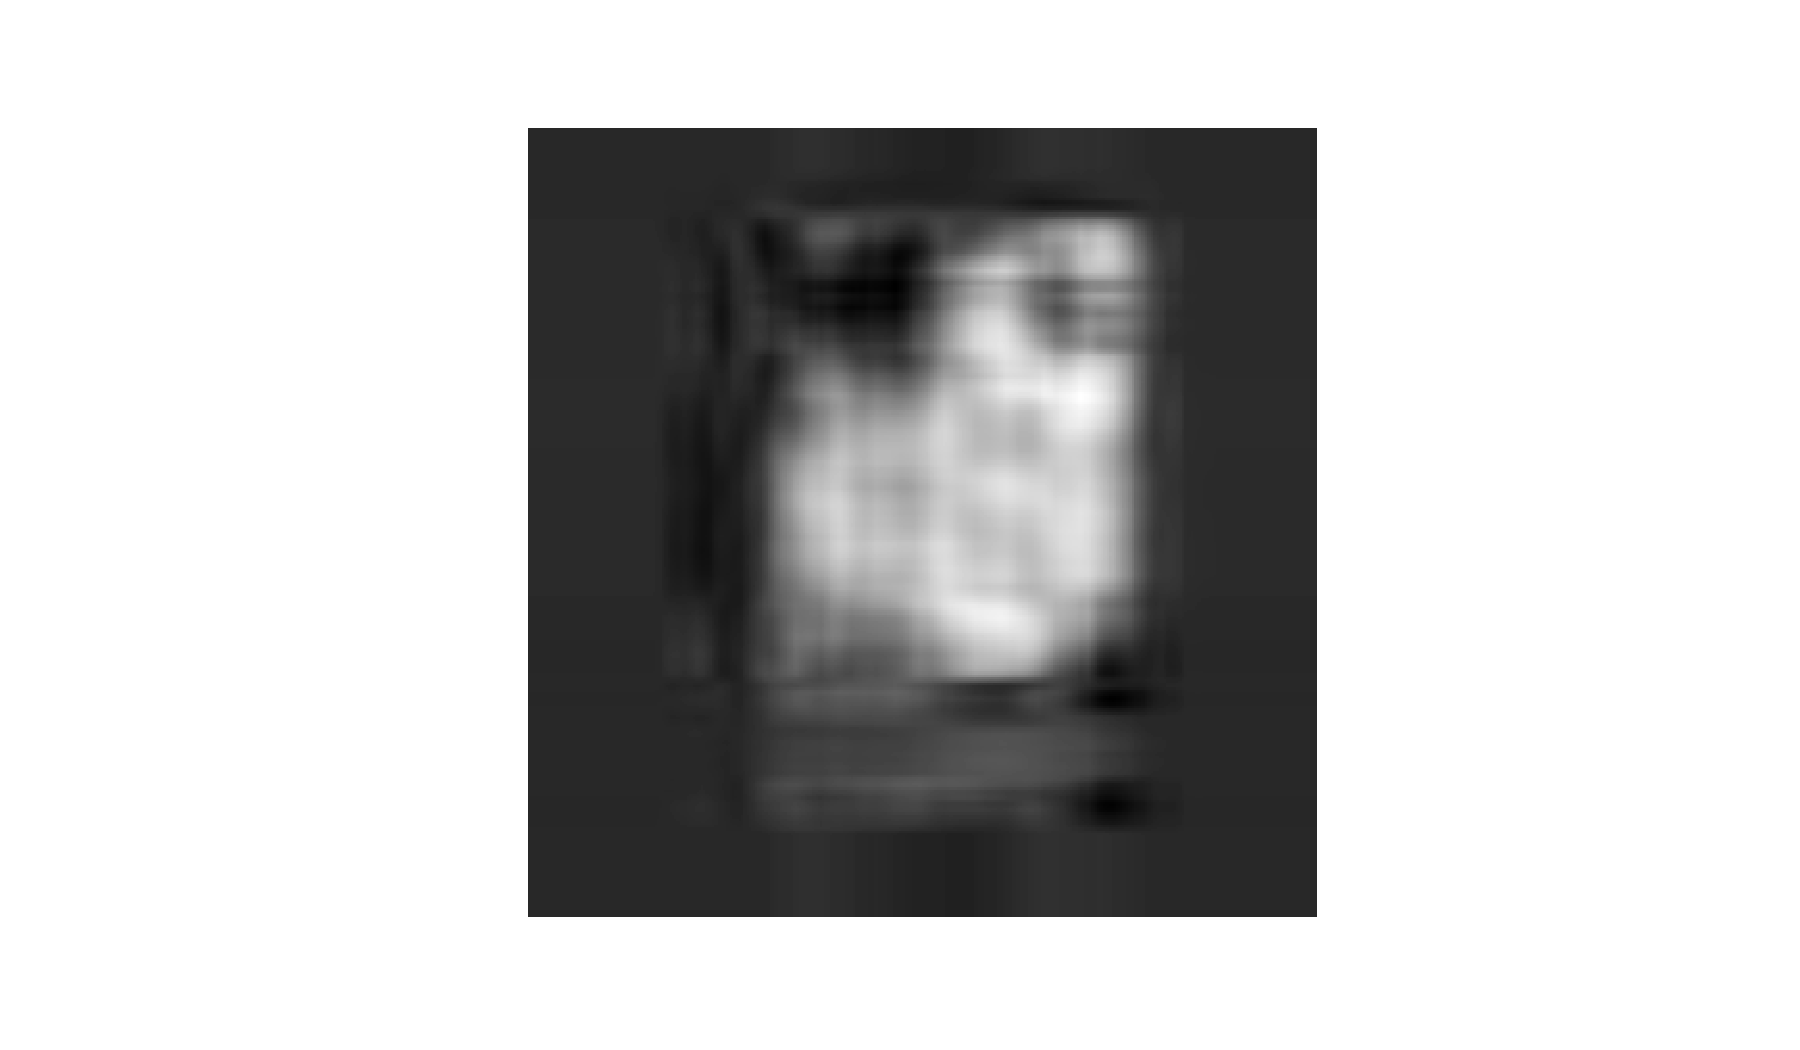
\includegraphics[width=0.32\textwidth]{../approx_8.pdf}} 
		\subfigure[]{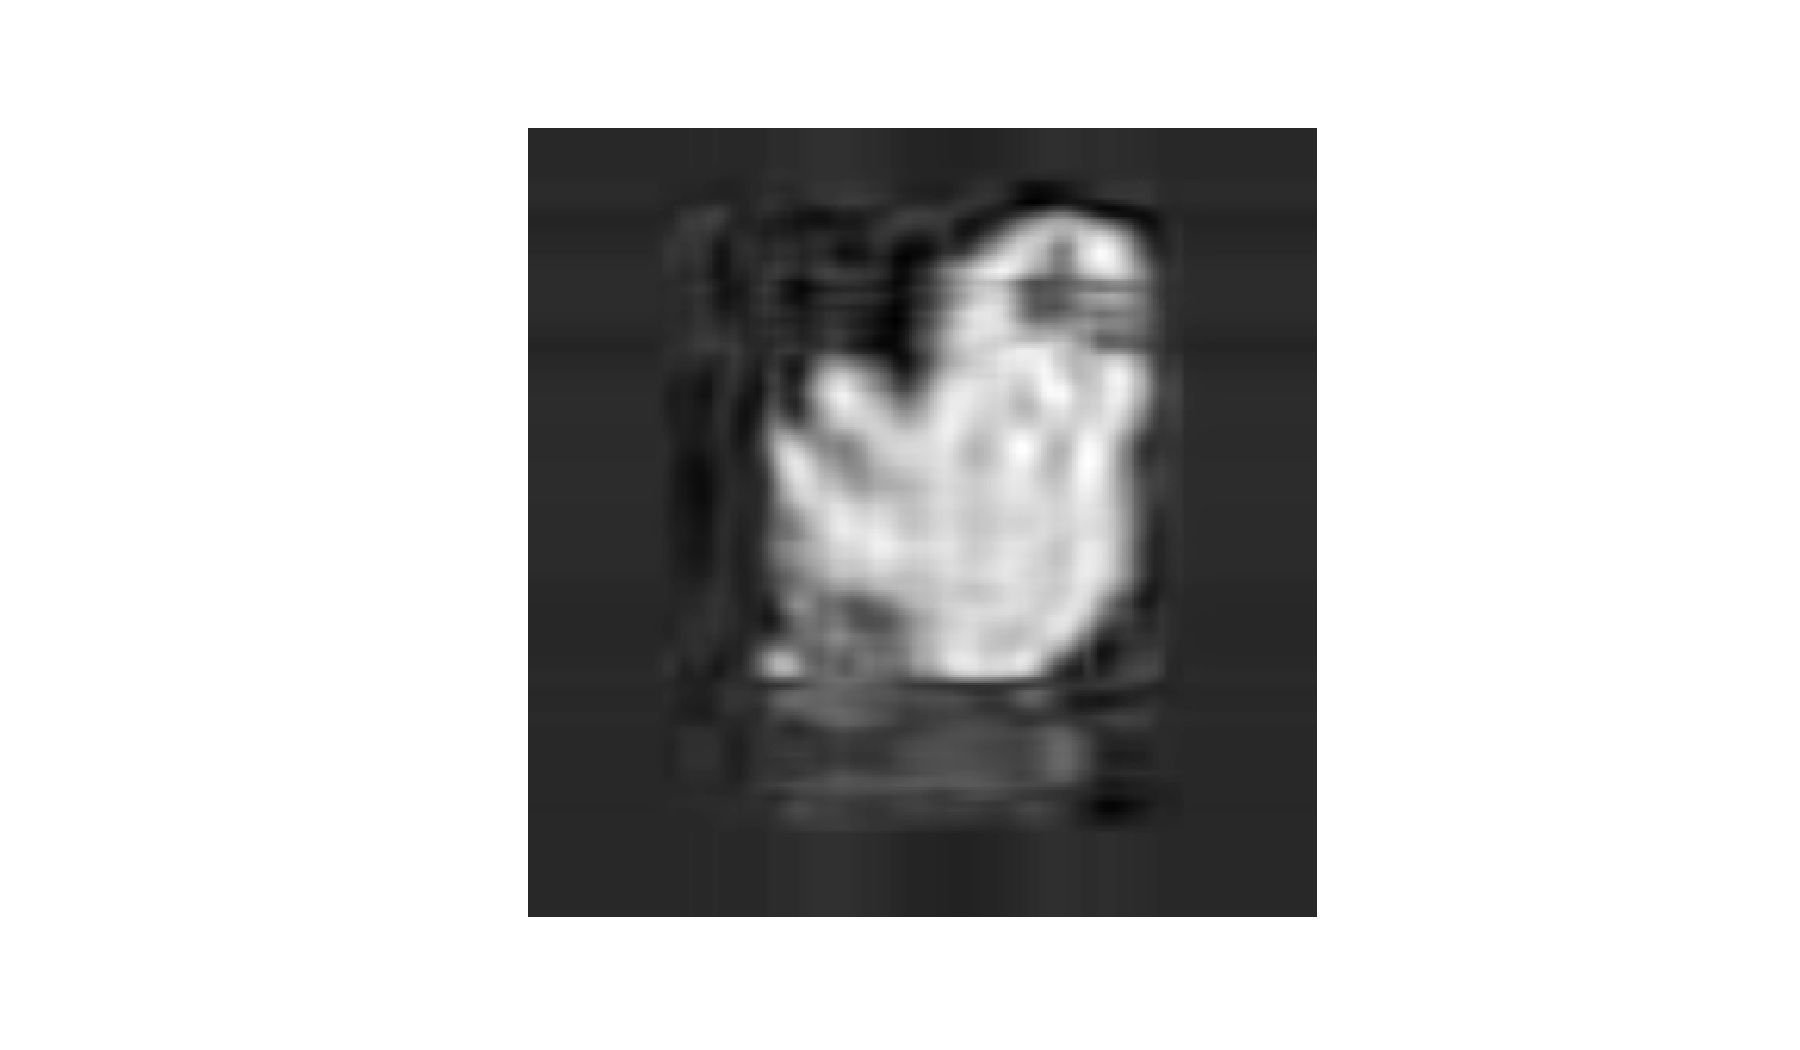
\includegraphics[width=0.32\textwidth]{../approx_12.pdf}}
		\subfigure[]{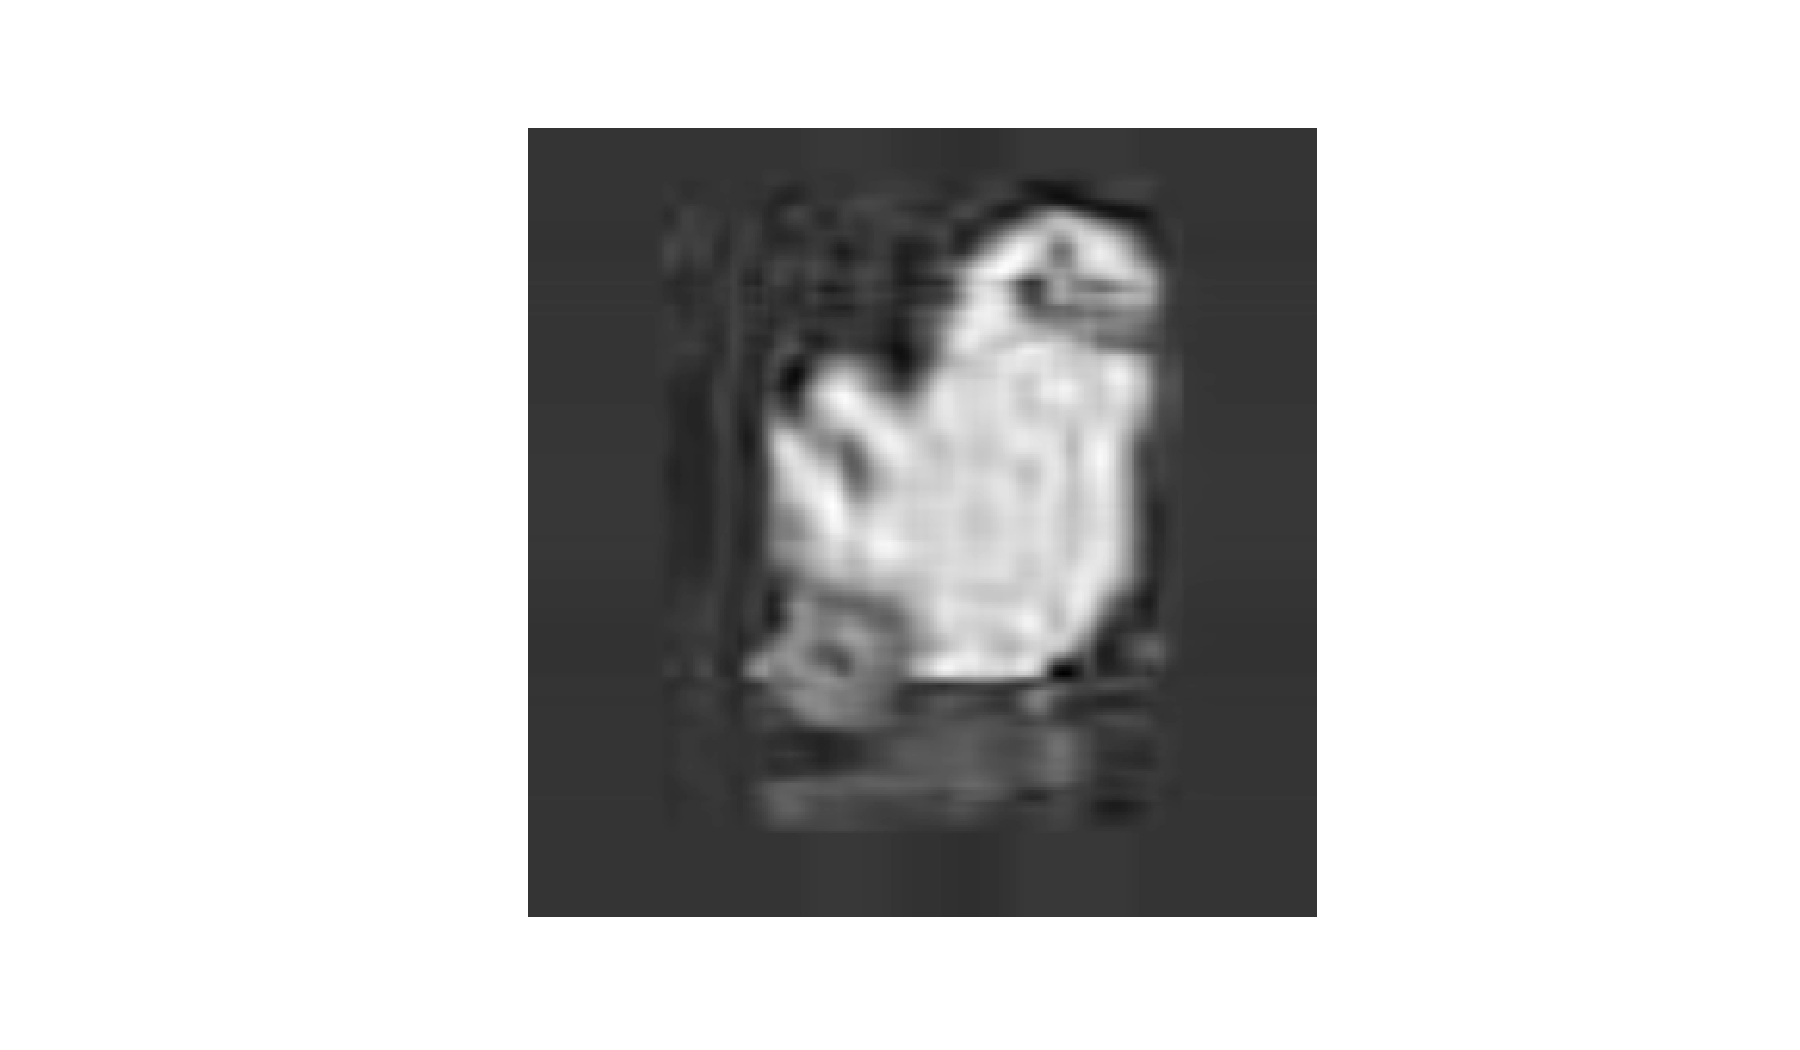
\includegraphics[width=0.32\textwidth]{../approx_16.pdf}}
		\subfigure[]{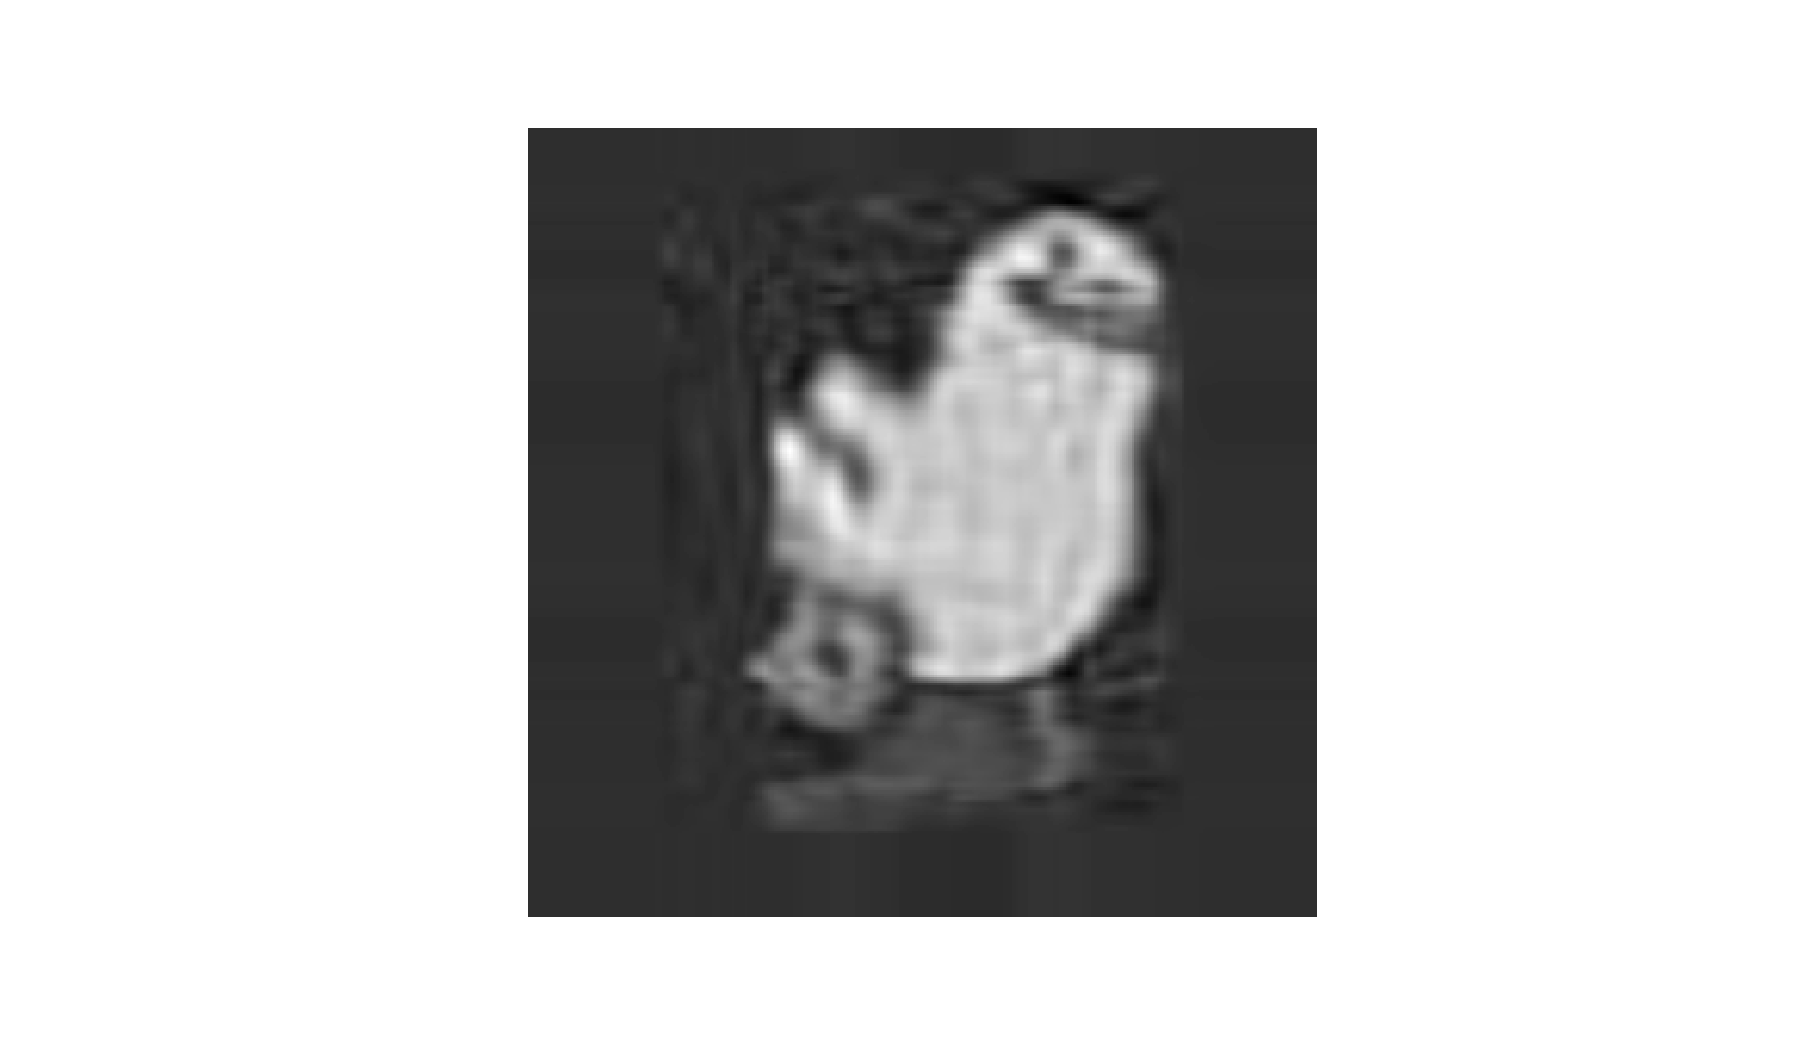
\includegraphics[width=0.32\textwidth]{../approx_20.pdf}}
		\subfigure[]{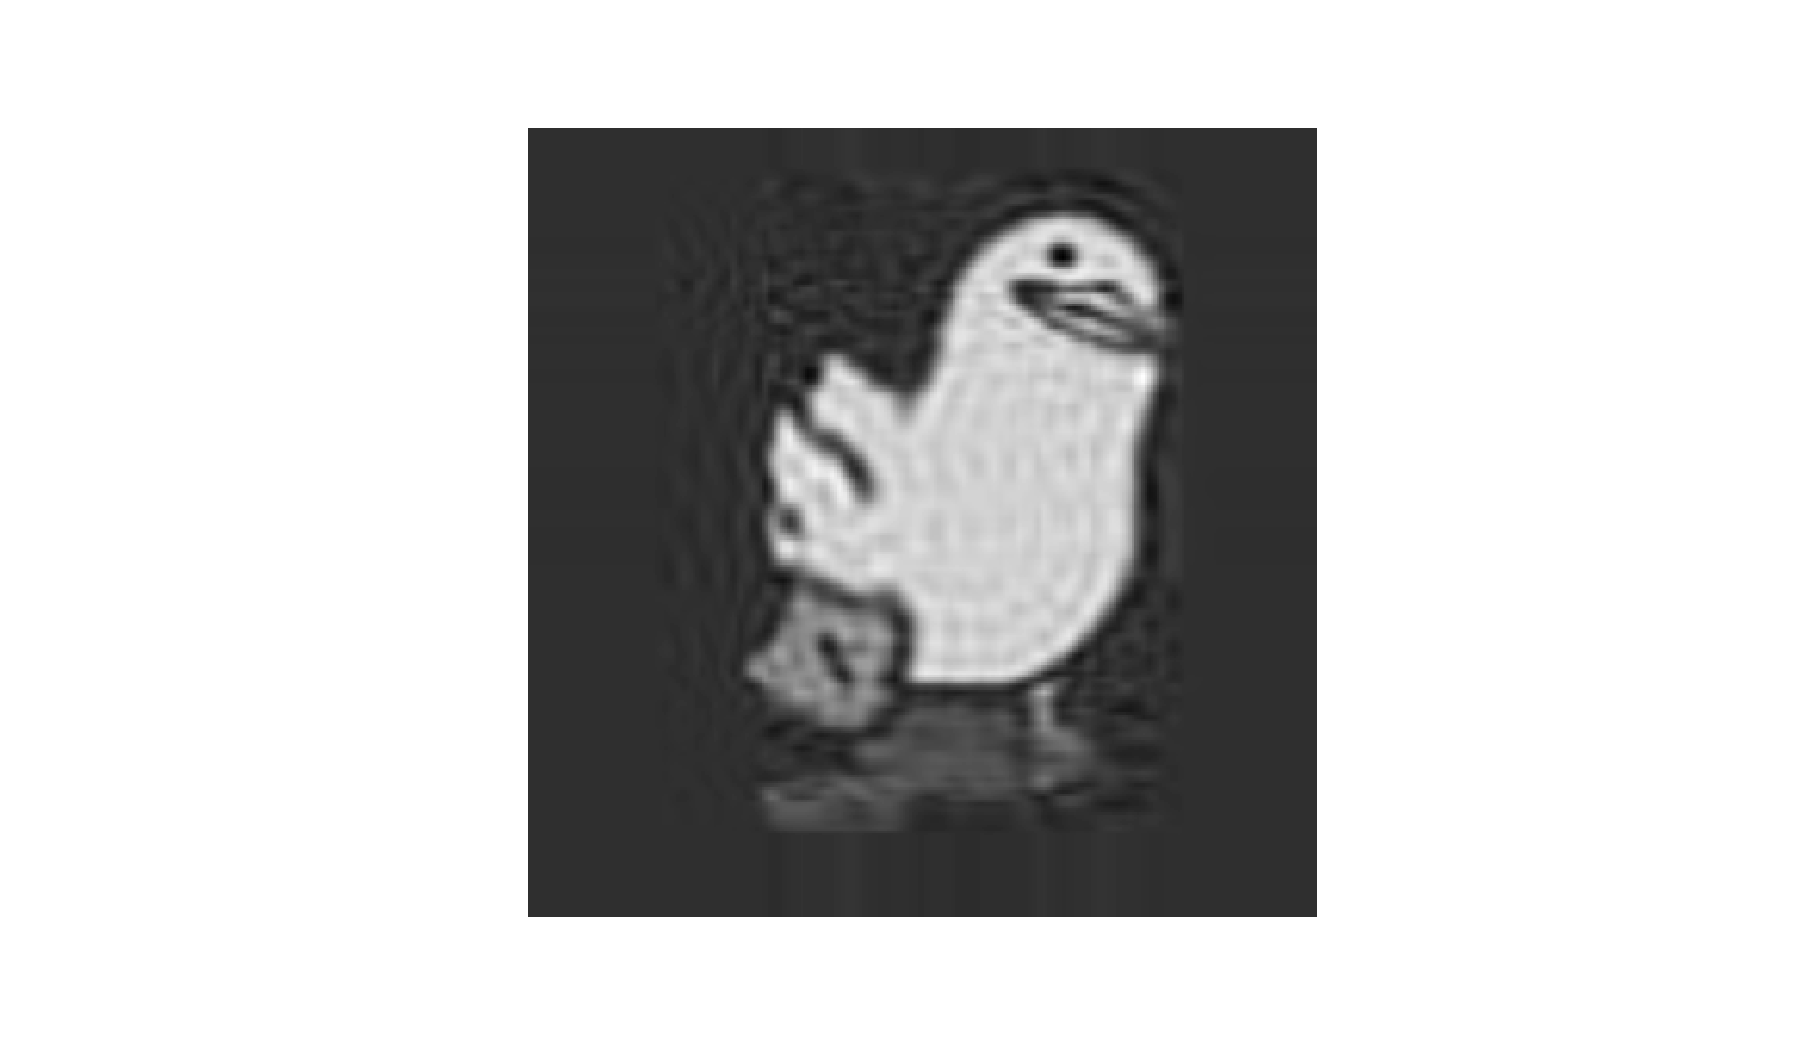
\includegraphics[width=0.32\textwidth]{../approx_32.pdf}}
		\subfigure[]{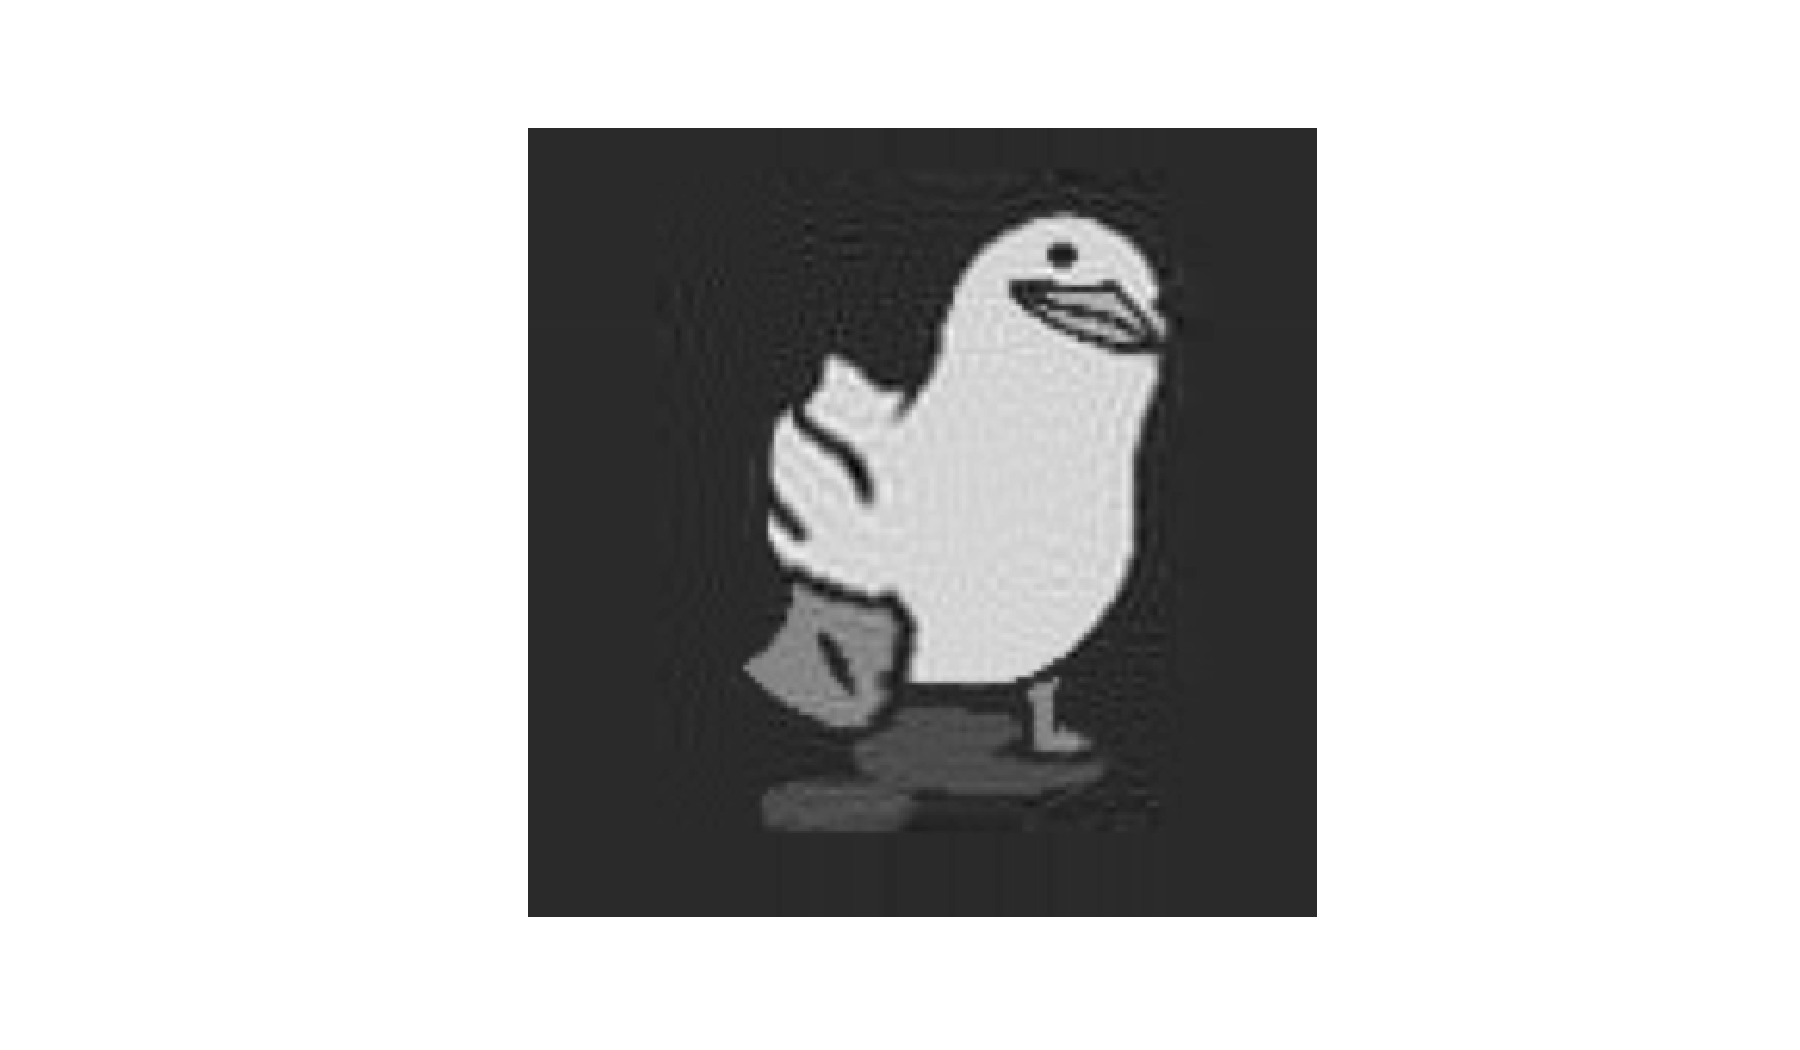
\includegraphics[width=0.32\textwidth]{../approx_64.pdf}}
		\subfigure[]{
\includegraphics[width=0.32\textwidth]{../approx_128.pdf}}
		\caption{Результат применения HOSVD с hid-size, равным (a) 4; (b) 8; (c) 12; (d) 16; (e) 20; (f) 32; (g) 64; (h) 128;}
		\label{fig:various_core_tensors}
	\end{figure}

	Было взято gif-изображение размером $128 \times 128$ и состоящее из $15$ кадров. 
	Далее продублировали сигнал $5$ раз, чтобы у нас был набор кадров из $5$ периодов. 
	
	После этого применяется HOSVD с core-тензорами разных размерностей $75 \times \text{hid-size} \times \text{hid-size}$ и восстанавливается аппроксимированный тензор. На рисунке \ref{fig:various_core_tensors} изображены исходное и восстановленные изображения. 
	Из аппроксимированного тензора составляется траекторная матрица картинок. 
	В качестве звукового сигнала $Y$ используется синусоида с периодом в $15$ шагов с добавленным нормальным шумом:
	\begin{gather*}
		Y = \left\{\sin\left(i * \frac{4 \pi}{15} \right) + \xi_i \right\}_{i=1}^{75} \text{, где } \xi_i \sim \mathcal{N}(0, 0.1^2)
	\end{gather*}
	
	К траекторным матрицам $\bH_X, \bH_Y$, полученным из аппроксимированного тензора $\uX$ и $Y$, применяется метод CCM. 
	
	Для каждого $i \in \{ 47, \ldots, 61 = (75-15+1)\}$ вычисляется $\varphi(\bH_Y[i])$. Для проверки на липшицевость в пр-вах $\dH_X$ и $\dH_Y$ использовались следующие метрики:
	$$ \rho_{\dH_Y}(y_1, y_2) = \| y_1 - y_2 \|_2, \quad \rho_{\dH_X}(x_1, x_2) = \| x_1 - x_2 \|_{\infty}.$$
	Уcтановлено, что при $C = 100$ отображение $\varphi$ является липшицевым (рисунки \ref{fig:dist_ratio_scatter}, \ref{fig:dist_ratio_table}).  
	
	Более того, корреляция между предсказаниями и исходными элементами траекторного пр-ва кадров превосходит $0.74$ (рисунок \ref{fig:corr_plot}).  
	
	Таким образом, можно заключить, что искомая причинная связь между временными рядами присутствует.
	
	\begin{figure}[bhtp]
		\centering
		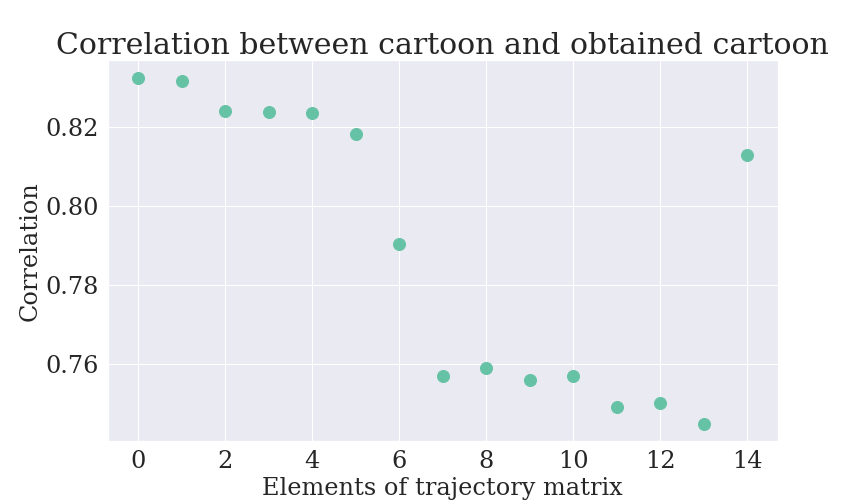
\includegraphics[width=\linewidth]{../correlation_plot.png}
		\caption{Корреляция между элементами траекторной матрицы кадров и предсказаниями, полученными с помощью метода ближайших соседей (функции $\varphi$)}
		\label{fig:corr_plot}
	\end{figure}

	\begin{figure}[bhtp]
		\centering
		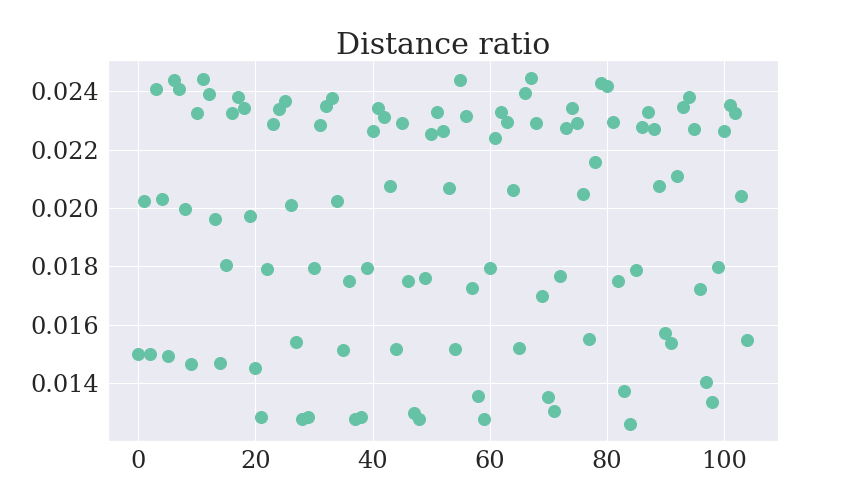
\includegraphics[width=\linewidth]{../dist_ratio_plot.png}
		\caption{Отношения расстояний (точечный график)}
		\label{fig:dist_ratio_scatter}
	\end{figure}

	\begin{figure}[bhtp]
		\centering
		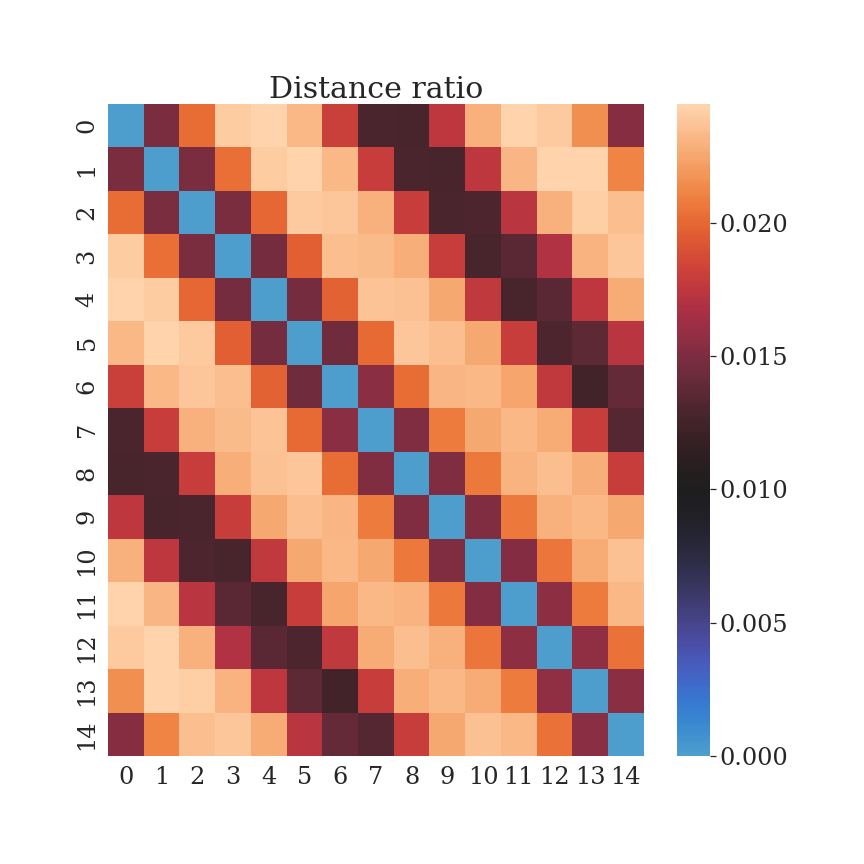
\includegraphics[width=\linewidth]{../dist_ratio_table.png}
		\caption{Отношения расстояний (таблица)}
		\label{fig:dist_ratio_table}
	\end{figure}

	\section{Литература}
	NULL
\end{document}
